
% \chapter{Reconstruction of musculoskeletal models using torque feasible sets}
\chapter{In silico musculoskeletal model reconstruction}
\label{chapter:4_old}
\usection{Introduction}
In a musculoskeletal model, muscles can be described as a succession of line segments. While there are other modelizations which involve polynomial descriptions (CITE), a segment model has the advantage of being computationally simpler to compute moment arms.

Hill-type muscle models consider three parameter categories. On one hand, there are \emph{geometric} parameters $\mathcal{X}_g$, which describe a muscle path surrounding bones and joints. There are also \emph{functional} parameters $\mathcal{X}_f$, allowing a modeling of all possible tension exertable by a muscle according to its length. In a Hill-type model, this includes the maximal isometric force $f_{iso}$, the optimal fiber length $l_{o}$ at which the muscle exert its maximal force $f_{iso}$, the tendon slack length $t_{sl}$, and the pennation angle $\alpha$.

This chapter focuses on finding a solution $\mathbf{x}^*$ such that:
$$\mathbf{x}^* = \argmin_{\mathbf{x}\in \mathcal{X}_g\times \mathcal{X}_f} \sum_{\mathbf{q}\in \mathcal{Q}} d(\mathcal{FE}(\mathbf{q}),\,\mathcal{F}(\mathbf{q}))$$

In other words, for experimentally measured maximal force exertion data gathered in an arbitrary amount of chosen postures, we want to find a set of musculoskeletal parameters such that the computed force feasible sets reproduce the measured data.

In this chapter, the measure maximal force exertion data are generated in silico, in order to grasp the best methods to solve this optimization. Next chapter \ref{chapter:5} focuses on in vivo data only.

Our approach is to gradually decrease our knowledge of all considered parameters in the optimization. This lead to a geometric understanding of the tension-moment relationship when considering all muscles as a single entity acting on joint torques. In other words, the underlying objective of this chapter is to understand the null space structure of a musculoskeletal model for force feasible set production. Characterizing the class of musculoskeletal models which produce the same force feasible sets allows us to reduce the search-space of the optimization.

In any case, we shall consider a fixed number of postures and that these postures are known, \emph{i.e.} $J^T(\mathbf{q})$ is always known. Each of the following cases are studied in this chapter:
\begin{itemize}
    \item {\textbf{Section 1:} for each produced maximal force exertion, associated muscle activations are known. This represent the best experimental conditions in which no assumption is made on the tension set modeling, all muscle activations are gathered, and produced forces at the end-effector are measured. We shall show that if muscles use a Hill-type muscle model, only three well-chosen postures are required and at least $m-(n-p)$ maximal force exertions are required per posture;}
    \item {\textbf{Section 2:} using a line segment cable model, torque feasible sets are known. It is assumed that the tension set is modelized as a $\mathcal{T}_{\infty}$ model - so we place ourselves in a purely robotic context. One advantage of this approach is the solving approach which is computed directly without any optimization. This approach extends to force feasible sets when no gravity is considered. In this case also, only two postures are required for reconstruction; }
    \item {\textbf{Section 3:} using a musculoskeletal model, force feasible sets are known under a $\mathcal{T}_{\infty}$ model. The reconstruction process uses a straight-forward approach with general solvers handling non-differentiability such as genetic algorithms and SRACOS;}
    \item {\textbf{Section 4:} using a musculoskeletal model, force feasible sets are known under a $\mathcal{T}_2$ model. ;}
\end{itemize} 

\begin{table}[!ht]
    \begin{tabular}{ccccccc}
     & \makecell{Tension \\ model} & \makecell{Known \\ tension values} & \makecell{Muscle \\ geometry} & \makecell{Force-length \\ relationship} & Solution & Applicable for                                             \\
    1       & Any $\mathcal{T}_p$         & Yes                  & Any             & Hill-Thelen               & Optimization & Force and torque feasible sets with gravity                \\
    2       & $\mathcal{T}_{\infty}$     & No                   & Lines    & Constant                  & Explicit     & Force (no gravity) and torque feasible sets (with gravity) \\
    3       & $\mathcal{T}_{\infty}$    & No                   & Any             & Hill-Thelen               & Optimization & Force and torque feasible sets with gravity                \\
    4       & $\mathcal{T}_2$          & No                   & Any             & Mean max & Optimization & Force and torque feasible sets with gravity               
    \end{tabular}
\end{table}

\section{Reconstructing cables from torque feasible sets}

The main goal of this section is to describe the set of all possible cables in a cable-driven parallel robot to produce force feasible sets in multiple joint configurations. In a sense, this section focuses on describing the geometric properties of a cable (attachment points) and its feasible tensions using only force and torque feasible sets.

The cable-driven parallel robots framework allows us to analyze the combinatorial challenges related to the possibilities as well as geometrically understand how. The main result is that the knowledge of torque feasible sets in only 3 joint configurations are required to identify the attachment points of a cable. A focus is also made onto the case where only 2 joint configurations are available.

Essentially, this step allows us to separate the geometric properties of a cable from its functional properties (tensions) in the torque space.

This section studies the geometric properties of torques feasible sets in order to find the set of all possible cables of a serial kinematic chain whose joints are actuated by rigid cables.

A \emph{cable-driven parallel robot} (CDPR) are ... definition (CITE LANDSBERGER , DARWIN LAU - CASPR).
This model includes rigid bodies and cables description.

\subsection{Cable-driven parallel robot formalism}
\paragraph*{Serial kinematic chain.} A serial kinematic chain consists of $k$ rigid bodies $B_1, \cdots, B_k$ linked successively via joints. For $i = 1, \cdots, k$, the joint between rigid bodies $B_{i-1}$ and $B_i$ describes the motion of body $B_i$ according to $B_{i-1}$. We denote this joint $J_i$. In particular, if it is assumed that the joint has a fixed center of rotation, we denote the center of joint $J_i$ by $P_i$. Since joint $J_i$ can induce rotational as well as translational motions, body $B_i$ has a relative orientation and translation according to $B_{i-1}$. To describe it, we define for each body $B_i$ a frame $\{F_i\}$ located at the body's center of mass $G_i$. When a joint configuration is fixed, it is thus possible to describe $B_i$'s frame and location according to the precedent $B_{i-1}$'s own frame and location through a rotation and translation mapping. For the first body $B_1$, its orientation and location are described according to the \emph{ground} notated $B_0$, which is assimilated to the origin of the space. The ground orientation and location are denoted $\{F_0\}$ and $O$ respectively. Figure \ref{fig:general_rigid_body_model} summarizes the serial kinematic chain formalism:
\begin{figure}[!htb]
    \captionsetup{justification=centering}
        \centering
        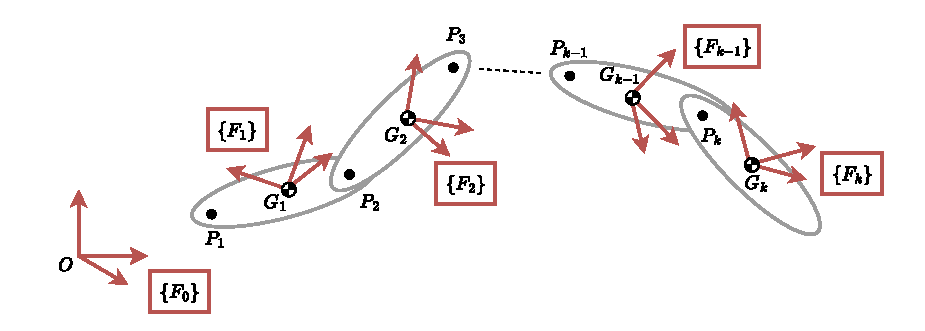
\includegraphics[trim={0 0 0 0},clip,width=1\linewidth]{img/chapter_4/general_rigid_body_model.pdf}
    \caption{Notations for a serial kinematic chain. The \emph{ground} $B_0$ is described via frame $\{F_0\}$ located at the origin $O$. A body $B_i$ is represented by a frame $\{F_i\}$ located at its center of mass $G_i$. Two bodies $B_{i-1}$ and $B_i$ are linked through a joint $J_i$ whose center is defined at point $P_i$. }
    \label{fig:general_rigid_body_model}
\end{figure}

\paragraph*{Joint motion.} A motion (also called \emph{displacement}) between two bodies $B_{i-1}$ and $B_i$ is the characterization of how $B_i$ can be displaced from $B_{i-1}$. In 3D, these displacements fall into three categories: (pure) translations, (pure) rotations and screw motions. A screw motion corresponds to a rotation and a translation occuring at the same time, resulting in a \emph{helical} motion. These displacements are invertible transformations.
\begin{figure}[!htb]
    \captionsetup{justification=centering}
        \centering
        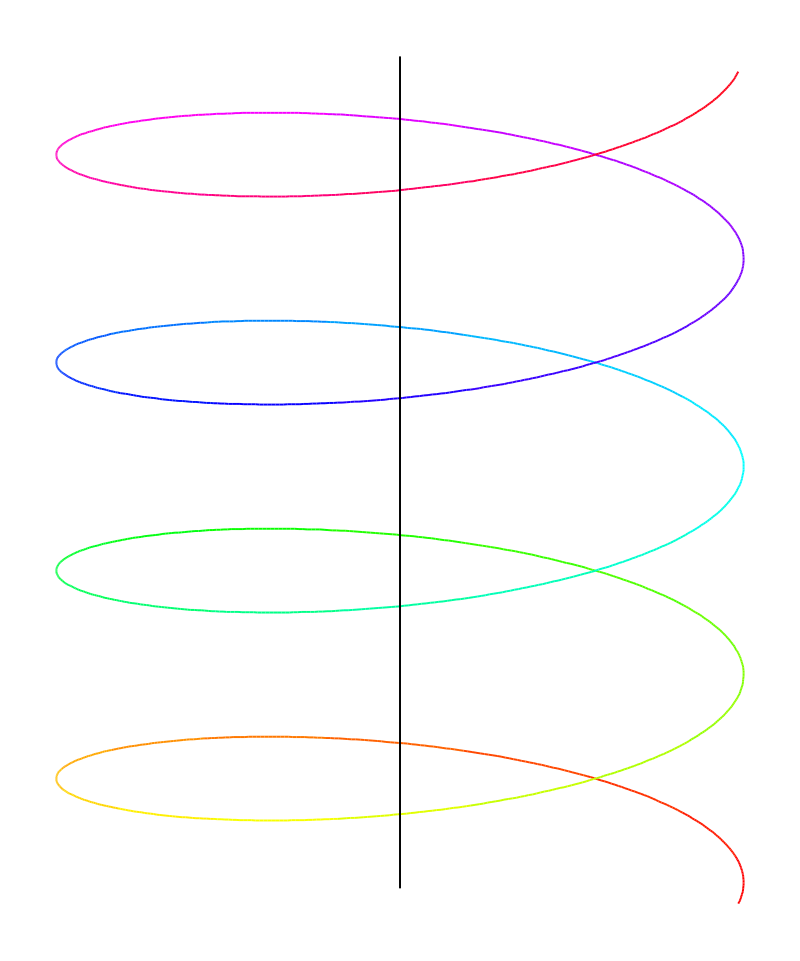
\includegraphics[trim={0 0 0 0},clip,width=0.3\linewidth]{img/chapter_4/screw_motion.png}
    \caption{A screw motion is the combination of a rotation and a translation occuring at the same time.}
    \label{fig:helical_motion}
\end{figure}

Translations occur along a direction vector $\mathbf{d}\in\IR^3$, whereas rotations occur around an \emph{axis} $\omega\in\IR^3$. Likewise, since screw motions consist of a rotation around axis $\omega$ and a translation about axis $\mathbf{d}$, they induce a motion around a \emph{screw axis} denoted $\mathbf{s} = (\mathbf{d}, \omega) \in \IR^6$.

A joint motion is thus characterized as a motion type and the representing element of the motion (vector for translations, axis for rotations and screw line for screw motions). 


\paragraph*{Degrees of freedom.} Motions are stable under composition of motions (two successive motions is a motion too), so it is convenient to describe a motion in a simpler motion decomposition. The \emph{degrees of freedom} of a motion refer to the number of independent axes or directions in which it can be decomposed. 

Since any translation in 3D can be described using three vectors, a translation motion has maximum 3 degrees of freedom. For rotation motions, Euler's rotation theorem states that any rotation in 3D can be represented as a rotation around a single axis. Since this axis is represented as a 3D vector, it can be described in a basis of 3 vectors or less. Thus, a rotation motion has maximum 3 degrees of freedom. A screw motion has consequently maximum 6 degrees of freedom, as it is a translation coupled with a rotation motion.

A joint whose underlying motion is a rotation motion of 3 DOFs is called a \emph{spherical joint}, whereas a translation motion of 3 DOFs is called a \emph{3 DOFs prismatic joint}.

\paragraph*{Generalized coordinates.} The \emph{generalized coordinates} of a motion are the parameters used to describe the configuration of a motion, and are denoted by a vector $\mathbf{q}\in\IR^p$ with $p$ the number of required parameters. For instance, a spherical joint has 3 generalized coordinates, whereas a \emph{revolute joint} (rotations around one axis only) has 1 generalized coordinates. A \emph{spatial joint} has a free screw motion (any translation and any rotation) so it is parametrized with 6 generalized coordinates.

In the previously defined serial kinematic chain, the generalized coordinates of each joint $J_i$ is denoted $\mathbf{q}_i\in\IR^{p_i}$ with $p_i$ the number of generalized coordinates for the motion of joint $i$. The generalized coordinates of the complete chain are concatenated in a vector $\mathbf{q}\in \IR^{p_1+p_2+\dots + p_k}$ following the definition order of the chain:
$$\mathbf{q} = \begin{bmatrix}
    \mathbf{q}_1 &  \mathbf{q}_2 & \dots & \mathbf{q}_k
\end{bmatrix}\in \IR^{p_1+p_2+\dots + p_k}$$


\paragraph*{Motors.} The transformation $M$ induced by a motion preserves the nature of a geometric object: a point is transformed into a point, a vector into a vector, a line into a line, a frame into a frame, a sphere into a sphere etc. This property has been extensively studied through the framework of \emph{geometric algebra}. While we do not describe the foundations of geometric algebra for consiveness purpose, we emphasize the properties of such transformations in order to avoid overbloated technicalities which are context-dependent.

We denote by $M_i(\mathbf{q})$ the invertible transformation called \emph{motor} induced from the motion of joint $J_i$ parametrized by $\mathbf{q}_i$. We recall that $\mathbf{q}_i$ is inscribed in $\mathbf{q}$. Explicit formulations of $M_i(\mathbf{q})$ are various and context-dependent: rotation matrix and translation vector, homogeneous transformations, rotor in geometric algebra, etc. Motors in $\IR^3$ can be:. So, in order to express in body $B_i$ a well-defined geometric entity $E_j$ initially expressed in body $B_j$ such that $i<j$, the following rule apply:
$$E_i = (M_i \circ M_{i+1} \circ \dots \circ M_{j-1} \circ M_j)(\mathbf{q})E_j = M_{ij}(\mathbf{q})E_j$$

Conveniently, as a shorthand to express a point, a vector or a normal vector in another frame of the serial kinematic chain, the right subscript notation is followed. For instance, we say \emph{point $P$ is expressed in body $B_k$} means that point $P$'s coordinates are drawn from frame $\{F_k\}$ located at center of mass $G_k$ and we precise it with the notation $P_{B_k}$. Similarly, \emph{point $P$ is expressed in joint $J_k$} refers to point $P$'s coordinates in the frame $\{F_{k-1}\}$ located at joint center $P_k$ and it is notated $P_{J_k}$.

\paragraph*{Cables.} A cable $C_{ij}$ is defined as a \emph{line segment}. In other words, it is a segment whose extremities are a point $O$ (the \emph{origin}) attached to body $B_i$ and a point $I$ (the \emph{insertion}) attached to body $B_j$. A cable exerts a positive pulling force (tension) along the direction going from $I$ to $O$. Let $l_{ij}(\mathbf{q})$ be the length of cable $C_{ij}$ for joint configuration $\mathbf{q}$. The cable tension $t$ is arbitrarily defined as a function of the cable length so that $t=t(l_{ij}(\mathbf{q}))$.
\begin{figure}[!htb]
    \captionsetup{justification=centering}
        \centering
        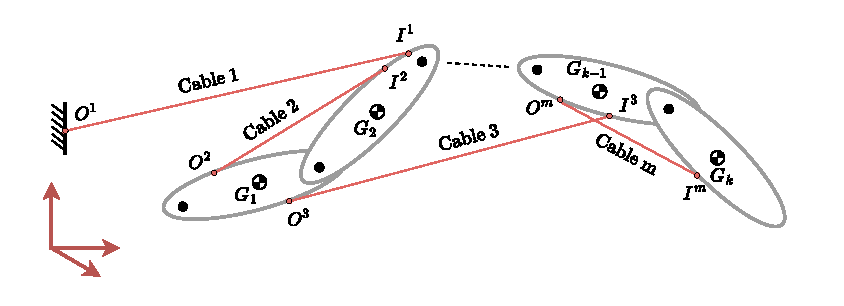
\includegraphics[trim={0 0 0 0},clip,width=1\linewidth]{img/chapter_4/cable_routing.pdf}
    \caption{}
    \label{fig:cable_routing}
\end{figure}

Since the equation of motion is expressed in the torque space, it is relevant to compute how muscle tensions are expressed in the torque space. Thus, the produced torques about or around each joint axis should be computed. Since the cable is designed to be a line segment, its produced force-moment are described by a force magnitude and the line geometry of the cable. So let's consider a cable $C_{ij}$, a joint $J_h$ and the torque $\tau$ produced by $C_{ij}$ about or around one of $J_h$ axes. First, we say that a cable $C_{ij}$ \emph{acts} on a joint $J_h$ if $i \leq h \leq j$. If $C_{ij}$ does not act on $J_h$, then it does not produce a torque about any of its axes and we have $\tau = 0$. If $C_{ij}$ acts on $J_h$, then if the considered axis is related to a rotational motion, we denote by $\omega$ this axis expressed in $J_h$ and we have
$$\tau = t\omega \cdot \left((O_{J_h} - P_h) \times \frac{O_{J_h} - I_{J_h}}{\| O_{J_h} - I_{J_h} \|} \right)$$
where $\cdot$ denotes the dot product and $\times$ the cross product. 
If the axis is related to a translational motion, we denote by $\mathbf{d}$ this axis expressed in $J_h$ and we have
$$\tau = t \mathbf{d} \cdot \frac{O_{J_h} - I_{J_h}}{\| O_{J_h} - I_{J_h} \|}$$

In a more general manner, the force and moment produced by cable $C_{ij}$ can be described as the Plücker coordinates of a line in different joint frames. This allows for a better geometric point of view of the cable produced torques. While $C_{ij}$ was defined using two bodies $B_i$, $B_j$ and two points $O$ and $I$ respectively expressed in each of them, it is relevant to ask ourselves it we could have chosen other $O$ and $I$ to produce the same torques. Essentially, one of our goal is to understand the null-space of the geometry of line segment cable. We will soon show that according to how the cable acts on joints, there may be an infinite amount of solutions or only one possible origin and insertion point (surprisingly). What matters is \emph{how structured is this infinite amount?} If we do know how it is structured, we better understand how to manipulate it.

\paragraph*{Plücker coordinates.}
One of our goal is to reconstruct a cable from its produced torques. We defined a cable to be a line segment, so it encapsulates the notion of \emph{line}. A line has various representations: two points (origin and insertion), Plücker coordinates, or intersection of two planes. Our approach focuses on Plücker coordinates, and directly use a conversion from the two-plane intersection description to obtain the two-points description. 

Let us have a more geometric approach of line segments. Consider a cable $C_{ij}$ as previous. Instead of considering a cable defined through two points, we shall consider a more unified representation of a line which allows us to describe in a same entity all lines formed by two distinct points drawn on $C_{ij}$. This representation is called \emph{Plücker coordinates}. A \emph{line} $L$ consists of two geometric concepts: an \emph{orientation} and a \emph{location}. The orientation of a line is defined to be the orientation of a vector (usually called \emph{direction}) passing through any two distinct points on $L$. It is thus assimilated to a vector $\mathbf{l}\in\IR^3$ of norm $1$. A direction behaves as a vector under motions, so that it is only affected by rotations, and translations do not have any impact on $\mathbf{l}$. The location part of a line $L$ is trickier to obtain: any point on $L$ could be used a location point. So we must find a way to describe it in a unique way. Let's first consider the vector $\mathbf{v}$ between a point $P$ and its orthogonal projection $P'$ onto $L$. The norm of $\mathbf{v}$ is called the \emph{lever arm of $L$ about point $P$}. However, in geometry, working with vectors is not always ideal since they are not affected by translations - so it is not useful for describing a change of frame for $L$. Let's consider an alternative approach: take a point $P$ and construct a sphere $S$ centered at $P$ of radius $\| \mathbf{v} \|$. This implies that $L$ intersects $S$ at $P'$. Consider the plane tangent to $S$ passing by $P'$: it is equivalent to consider the plane normal to $\mathbf{v} / \| \mathbf{v} \|$ passing through $P'$. Now, this planes has a redundant information: it contains the direction part of $L$. Even though it is not necessarily computable directly from the plane description, we do know that the direction will necessarily influence the location and orientation of the tangent plane. We thus concentrate on the element which describes the plane and resemble the less the direction of $L$: this corresponds to the normal vector $m\in\IR^3$ to the plane formed by the direction vector $\mathbf{d}$ and the vector $\mathbf{v}$. This normal vector is called \emph{moment of the line $L$}. Note that it is a \emph{normal}, so it is impacted by translational motions. By construction, notice also that $\mathbf{l} \cdot m = 0$, when we consider $m$ as a vector.

The Plücker coordinates of $L$ are thus:
$$L = (\mathbf{l};\, m)$$
with $\mathbf{l}\in\IR^3$ a unit vector (direction) and $m\in\IR^3$ a normal vector (moment). The direction encodes the orientation of $L$, whereas the moment encodes its location. Plücker coordinates are a compact description of a line, whose components behave nicely under motions: this means we have an easy tool to describe a cable with change of frames. As a side-note, Pücker coordinates may seem similar to the notion of \emph{wrench} or \emph{twist}: this is because they \emph{are} based on Plücker coordinates.

For instance, to describe the force and torque of a cable $C_{ij}$ described in the joint frame $J_h$, consider a cable tension of $t>0$ Newton and $\delta_{J_h} = 0$ if $C_{ij}$ does not act on $J_h$ or $\delta_{J_h} = 1$ otherwise.
Define the cable wrench $\mathbf{w} = \delta_{J_h} t L_{J_h} = (\delta_{J_h} t\mathbf{l}_{J_h};\, \delta_{J_h} t m_{J_h})$. The wrench is thus a line object with a weight $\delta_{J_h} t$.

\subsection{Origin and insertion points of a cable from its torques}
Consider a serial kinematic chain as previously defined. We assume that each joint induces either a 3 DOFs rotation motion or 3 DOFs translation motion, or 6 DOFs screw motion.

Suppose that a cable $C_{ij}$ exerts wrench $\mathbf{w}(\mathbf{q})$ at joint configuration $\mathbf{q}$, and assume the knowledge of its wrench about or around axes. We recall that the produced torques for joint $J_h$, notated $\tau_{J_h}$, correspond to formula (CF ABOVE).

\paragraph*{Finding origin and insertion bodies.}
If $C_{ij}$ does not act on joint $J_h$, then $\tau_{J_h} = 0$. Using the serial construction of the kinematic chain, we retrieve the origin and insertion point bodies of $C_{ij}$ via algorithm \ref{alg:find_bodies_origin_insertion} which returns the possible bodies of origin and insertion. These possible bodies are the first and last bodies in the kinematic chain such that the produced torques are not null. 
\begin{figure}[!ht]
    \centering
    \begin{minipage}{1.0\linewidth}
        \begin{algorithm}[H]
            \SetAlgoLined
            \KwData{$\tau_{J_1},\dots,\tau_{J_k}$ the produced torques of a cable ordered according to the serial structure of the kinematic chain}
            \KwResult{$B_i$ the body of the origin and $B_j$ the body of the insertion point}
            
            \SetKwFunction{FMain}{possibleBodiesOriginInsertion}
            \SetKwProg{Fn}{Function}{:}{}
            \Fn{\FMain{$\textup{E}_d$}}{
                $B \gets \emptyset$\;
                \ForEach{$\tau_{J_h}\in [\tau_{J_1},\dots,\tau_{J_k}]$}{
                    \If{$\tau_{J_h} != \mathbf{0}$}{
                        $B \gets B\cup \{B_h\}$\;
                    }
                }
                \Return{$\textup{E}_{d+1}$}
            }
            \textbf{End Function}
            \caption{Possible bodies for the origin and insertion points of a cable}
            \label{alg:find_bodies_origin_insertion}
        \end{algorithm}
    \end{minipage}
\end{figure}

One case which is not taken into account here is the situation in which the cable passes \emph{exactly} at the center of a rotational joint. In this case, the produced torque is null since expressed in this joint, the cable location is at the joint origin. However, it can be argued that mechanically no rigid cable can pass exactly through the center of a joint.

Another problem is to associate one of the two bodies with either the origin or insertion point. We will see that a solution can be found a bit later.

\subsubsection{Origin and insertion of cable acting on one rotational joint}
Let's consider two joint configurations $\mathbf{q}_1$ and $\mathbf{q}_2$. Let $C_{ij}$ be a cable acting on one rotational joint $J_h$ only. Denote by $\omega_1(\mathbf{q})$, $\omega_2(\mathbf{q})$ and $\omega_3(\mathbf{q})$ its rotation axes expressed in the joint for joint configuration $\mathbf{q}$. Let $t(\mathbf{q}) > 0$ be the exerted tension of cable $C_{ij}$. $C_{ij}$ is a line segment, so let $L(\mathbf{q}) = (\mathbf{l}(\mathbf{q}) : \mathbf{m}(\mathbf{q}))$ be the Plücker coordinates of its underlying line generated by its origin and insertion point expressed in joint $J_h$ at joint configuration $\mathbf{q}$.

Its produced torques $\tau\in\IR^3$ on $J_h$ at joint configuration $\mathbf{q}$ are thus 
\begin{align*}
    \begin{pmatrix}
        \tau_1(\mathbf{q}) \\
        \tau_2(\mathbf{q}) \\
        \tau_3(\mathbf{q})
    \end{pmatrix} = \begin{pmatrix}
        \omega_1(\mathbf{q}) \cdot t(\mathbf{q})\mathbf{m}(\mathbf{q}) \\
        \omega_2(\mathbf{q}) \cdot t(\mathbf{q})\mathbf{m}(\mathbf{q}) \\
        \omega_3(\mathbf{q}) \cdot t(\mathbf{q})\mathbf{m}(\mathbf{q})
    \end{pmatrix}
\end{align*}
Let $\Omega(\mathbf{q}) = \begin{pmatrix}
    \omega_1^T(\mathbf{q}) \\
    \omega_2^T(\mathbf{q}) \\
    \omega_3^T(\mathbf{q})
\end{pmatrix} \in \IR^{3\times 3}$ and $\tau(\mathbf{q}) = (\tau_1(\mathbf{q}), \tau_2(\mathbf{q}), \tau_3(\mathbf{q}))\in \IR^3$. 
Since $J_h$ generates a 3D rotational motion, each of the axis (expressed in the joint frame) are non-colinear so that $\Omega$ is invertible. We thus have
\begin{align*}
    \tau(\mathbf{q}) &= t(\mathbf{q})\Omega(\mathbf{q})\mathbf{m}(\mathbf{q}) \\
    \iff \Omega(\mathbf{q})^{-1}\tau(\mathbf{q}) &= t(\mathbf{q})\mathbf{m}(\mathbf{q})
\end{align*}
This expression implies that the origin and insertion point, expressed in the joint frame, belongs to the plane passing through the joint center and of normal vector $\Omega(\mathbf{q})^{-1}\tau(\mathbf{q})$. Let's denote $P(\mathbf{q})$ this plane expressed in $J_h$, $P_{B_i}(\mathbf{q})$ this plane expressed in the origin point body and $P_{B_j}(\mathbf{q})$ this plane expressed in the insertion point body. We thus have the following:
\begin{align*}
    & O_{J_h}\in P(\mathbf{q}) \quad \text{and} \quad I_{J_h}\in P(\mathbf{q}) \\
    \iff & O\in P_{B_i}(\mathbf{q}) \quad \text{and} \quad I\in P_{B_j}(\mathbf{q})
\end{align*}



The definition of the moment $\mathbf{m}$ of a line $L = (\mathbf{l} : \mathbf{m})$ implies that any point on $L$ belongs to the plane of normal $\mathbf{m}$ and passing through the origin of the considered frame of expression. This plane is noted $\mathbf{m}^*$\footnote{The notation $\mathbf{m}^*$ references the Hodge dual operator ${}^*$: it is a stronger notion of orthogonality, which preserves orientation. While we do not dive into the details of this duality, it is useful in its notation and consiveness and can be (roughly) summarized as a generalization of the link made between a normal and a plane, but also the link between a rotation axis and a plane of rotation. Also, with a bit of rewritting using \emph{geometric algebra} and generalized Plücker coordinates, all presented results generalize to any dimension (for full-dimensional rotational joints of a n-dimensional serial kinematic chain equipped with cables as line segments). Since it would require to present the geometric algebra framework in details for not-so-interesting results, we shall skip the generalization. The reader can get acquainted with \emph{geometric algebra} in \cite{dorstGeometricAlgebraComputer2007}.}.

\begin{theorembox}{Time complexity of EdgeEnum}{rotational_solution_moment}
    Consider a serial kinematic chain consisting of $k$ rigid bodies $B_1, \dots, B_k$ linked successively through $k$ rotational joints $J_1, \dots, J_k$ of 3 degrees of freedom. For $h=1,\dots, k$, each joint $J_h$ is parametrized by generalized coordinates $\mathbf{q}_{J_h} = (q_{J_h}^1, q_{J_h}^2, q_{J_h}^3)\in [-\pi, \pi]^3$ and its rotation axes, expressed at the joint center of rotation, are denoted $\omega_{J_h}^1, \omega_{J_h}^2$ and $\omega_{J_h}^3$. Consider a line segment cable $C_{ij}$ of attachment points $O_{B_i}$ and $I_{B_j}$ acting on joints $J_h$ for $i< h\leq j$.

    $\tau_{C_{ij}}^h = $
\end{theorembox}


Consider a serial kinematic chain consisting of $k$ rigid bodies $B_1, \dots, B_k$ linked successively through $k$ rotational joints $J_1, \dots, J_k$ of 3 degrees of freedom. For $h=1,\dots, k$, each joint $J_h$ is parametrized by generalized coordinates $\mathbf{q}_{J_h} = (q_{J_h}^1, q_{J_h}^2, q_{J_h}^3)\in [-\pi, \pi]^3$ and its rotation axes, expressed at the joint center of rotation, are denoted $\omega_{J_h}^1, \omega_{J_h}^2$ and $\omega_{J_h}^3$. 


\begin{theorembox}{3 DOFs prismatic joint}{prismatic3D_solution}
    Consider a line segment cable $C_{ij}$ of attachment points $O_{B_i}$ and $I_{B_j}$ acting on a 3 DOFs prismatic joint $J_h$. Let $\mathbf{q}_1$ and $\mathbf{q}_2$ be two joint configurations and denote $\tau(\mathbf{q})\in\IR^3$ the produced torques in joint configuration $\mathbf{q}$. Then we have

    \begin{itemize}
        \item {for two joint configurations $\mathbf{q}_1$, $\mathbf{q}_2$, there is an infinite amount of locations for $O_{B_i}$ and $I_{B_j}$;}
        \item {For three joint configurations, $O_{B_i}$ and $I_{B_j}$ are uniquely determined by $\tau(\mathbf{q}_1)$, $\tau(\mathbf{q}_2)$ and $\tau(\mathbf{q}_3)$.}
    \end{itemize}
\end{theorembox}
\begin{proof}
    
\end{proof}


\begin{theorembox}{3 DOFs prismatic joint}{prismatic3D_solution}
    Consider a line segment cable $C_{ij}$ of attachment points $O_{B_i}$ and $I_{B_j}$ acting on a 3 DOFs prismatic joint $J_h$. Let $\mathbf{q}_1$ and $\mathbf{q}_2$ be two joint configurations and denote $\tau(\mathbf{q})\in\IR^3$ the produced torques in joint configuration $\mathbf{q}$. Then if we have three joint configurations, $O_{B_i}$ and $I_{B_j}$ are uniquely determined by $\tau(\mathbf{q}_1)$, $\tau(\mathbf{q}_2)$ and $\tau(\mathbf{q}_3)$.
\end{theorembox}
\begin{proof}
    Let $D_{J_h} = \begin{pmatrix}
        \mathbf{d}_{J_h}^x & \mathbf{d}_{J_h}^y & \mathbf{d}_{J_h}^z
    \end{pmatrix}\in \IR^{3\times 3}$ be the matrix containing the three translation axes of joint $J_h$ as columns. Since $J_h$ is a 3 DOFs prismatic joint, $D_{J_h}$ is invertible. Let $\mathbf{u}_{J_h}(\mathbf{q})\in\IR^3$ be the unit vector representing the direction of cable $C_{ij}$ expressed in joint $J_h$ for joint configuration $\mathbf{q}$. Then,
    \begin{align*}
        \tau_{J_h}(\mathbf{q}) &= t(\mathbf{q})D_{J_h}\mathbf{u}_{J_h}(\mathbf{q}) \\
        \iff D_{J_h}^{-1}\tau_{J_h}(\mathbf{q}) &= t(\mathbf{q})\mathbf{u}_{J_h}(\mathbf{q})
    \end{align*}

    By denoting $\mathbf{v}_{J_h}(\mathbf{q}) = D_{J_h}^{-1}\tau_{J_h}(\mathbf{q})$, we have 
    $$I_{J_h} = O_{J_h} + \lambda(\mathbf{q}) \mathbf{v}_{J_h}(\mathbf{q})$$

    By detailing $O_{J_h} = R_{ih}(\mathbf{q})O + t_{ih}(\mathbf{q})$ and $I_{J_h} = R_{jh}(\mathbf{q})I + t_{jh}(\mathbf{q})$, we have

    \begin{align*}
        R_{jh}(\mathbf{q})I + t_{jh}(\mathbf{q}) - R_{ih}(\mathbf{q})O - t_{ih}(\mathbf{q}) &= \lambda(\mathbf{q})\mathbf{v}(\mathbf{q}) \\
        \iff R_{jh}(\mathbf{q})I  - R_{ih}(\mathbf{q})O - \lambda(\mathbf{q})\mathbf{v}(\mathbf{q}) &= - t_{jh}(\mathbf{q}) + t_{ih}(\mathbf{q}) \\
        \iff \begin{bmatrix}
            - R_{ih}(\mathbf{q}) & R_{jh}(\mathbf{q}) & -\mathbf{v}(\mathbf{q})
        \end{bmatrix}\begin{bmatrix}
            O \\ I \\ \lambda(\mathbf{q})
        \end{bmatrix} &= - t_{jh}(\mathbf{q}) + t_{ih}(\mathbf{q})
    \end{align*}

    Let $A \in \IR^{9\times 9}$ be the matrix 
    $$A = \begin{bmatrix}
        - R_{ih}(\mathbf{q}_1) & R_{jh}(\mathbf{q}_1) & -\mathbf{v}(\mathbf{q}_1) & \mathbf{0} & \mathbf{0} \\
        - R_{ih}(\mathbf{q}_2) & R_{jh}(\mathbf{q}_2) & \mathbf{0} & -\mathbf{v}(\mathbf{q}_2) & \mathbf{0} \\
        - R_{ih}(\mathbf{q}_3) & R_{jh}(\mathbf{q}_3) & \mathbf{0} & \mathbf{0} & -\mathbf{v}(\mathbf{q}_3)
    \end{bmatrix}$$
    and $\mathbf{b}\in\IR^9$ the vector
    $$\mathbf{b} = \begin{pmatrix}
        -t_{jh}(\mathbf{q}_1) + t_{ih}(\mathbf{q}_1) \\
        -t_{jh}(\mathbf{q}_2) + t_{ih}(\mathbf{q}_2) \\
        -t_{jh}(\mathbf{q}_3) + t_{ih}(\mathbf{q}_3)
    \end{pmatrix}$$

    Then the problem is written as follows:
    \begin{align}
        \label{eq:Axb}
        A\begin{bmatrix}
            O \\ I \\ \lambda(\mathbf{q}_1) \\ \lambda(\mathbf{q}_2) \\ \lambda(\mathbf{q}_3)
        \end{bmatrix} = \mathbf{b}
    \end{align}

    If $A$ is invertible, then there is a unique solution to equation \ref{eq:Axb}.
\end{proof}


\begin{theorembox}{Spherical joint}{spherical_joint_theorem}
    Let $J_h$ be a spherical joint and denote $\omega_1(\mathbf{q})$, $\omega_2(\mathbf{q})$, $\omega_3(\mathbf{q})\in \IR^3$ be its rotations axes expressed in $J_h$ frame. 

    For a cable $C_{ij}$, let $\tau(\mathbf{q})\in\IR^3$ be its exerted torque onto joint $J_h$.

    If $i \neq h$ and $j \neq h$, then $O$ and $I$ are uniquely determined by $\tau(\mathbf{q})$ known for three joint configurations.

    If $h = i$ or $h = j$, then the set of possible lines is infinite and is parametrized by a doubly ruled surface.
\end{theorembox}
\begin{proof}
    \textunderscore{ok}
\end{proof}

\subsubsection*{Spherical joint}

\usubsection{Upper-limb musculoskeletal model of reference}


\usubsection{Muscle path and muscle tension modeling}
\usubsection{Torque feasible set modeling for a small or large amount of muscles}
\usubsection{Force feasible set modeling for a small or large amount of muscles}
\usubsection{Optimization-based and geometry-based approaches}
\usubsection{Derivative-free solvers}
\usubsection{On the number of required postures}

\section{Reconstruction process based on torque feasible sets}
\subsection{Considering a small amount of muscles}
\usubsubsection{Using muscles with constant tensions}
\usubsubsection{Using Hill-type muscles}
\subsection{Considering a large amount of muscles}
\usubsubsection{Using muscles with constant tensions}
\usubsubsection{Using Hill-type muscles}

\section{Reconstruction process based on force feasible sets}
\subsection{Considering a small amount of muscles}
\usubsubsection{Using muscles with constant tensions}
\usubsubsection{Using Hill-type muscles}

\subsection{Considering a large amount of muscles}
\usubsubsection{Using muscles with constant tensions}
\usubsubsection{Using Hill-type muscles}
\section{Results and discussion}
\usection{Conclusion}